\documentclass{article}

\usepackage[utf8]{inputenc}
\usepackage[T1]{fontenc}
\usepackage[francais]{babel}
\usepackage{graphicx}
\usepackage{multicol}
\usepackage[top=1cm,left=1cm,right=1cm,bottom=1cm]{geometry}
\usepackage{wrapfig}
\usepackage{vwcol}

\begin{document}

\section{Mission A}

\subsection{Sous-Mission A4}

\begin{vwcol}[widths={0.8,0.2}, rule=0pt]
\begin{minipage}{0.7\textwidth}
\paragraph{Objectifs de la mission}

Rendre une image de la planète Jupiter plus nette. Pour se faire nous avions à disposition deux photographies faites à quelques secondes d'intervalle comprenant toutes deux du bruit.
\end{minipage}
\begin{minipage}{0.3\textwidth}
\begin{flushright}
\paragraph{Téchniques utilisés}

Soustraction \& Filtre médiant
\end{flushright}
\end{minipage}
\end{vwcol} 

\begin{figure}[h]
\centering
	\begin{multicols}{2}
	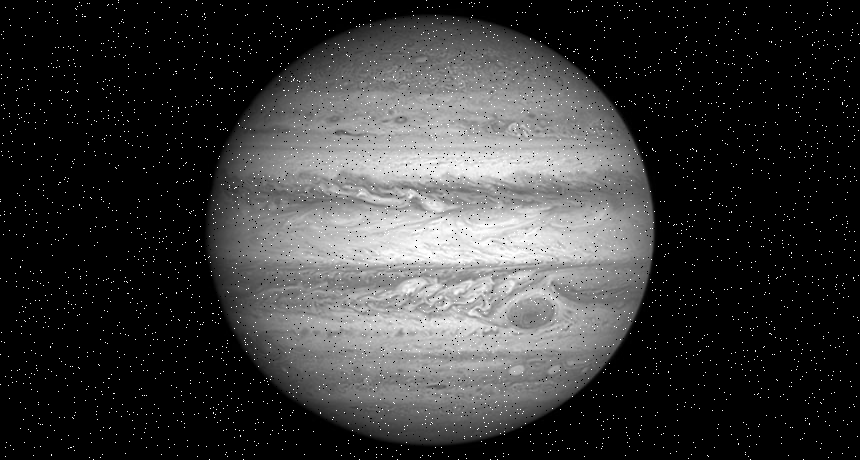
\includegraphics[scale=0.325]{img/Jupiter.png}
	Avant
	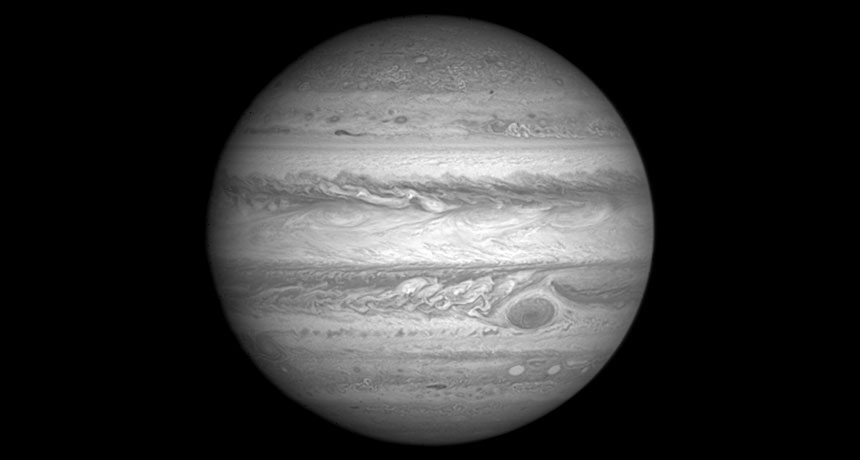
\includegraphics[scale=0.325]{img/JupiterAp.png}
	Apres
	\end{multicols}
	\vspace{-0.9cm}
	\caption{Résultat de la mission A4}
	\label{A4}
\end{figure}

\paragraph{Procédé}

Le résultat ci-dessus, nous avons utilisé deux filtes à la suite. Tout d'abord, nous avons \emph{soustrait} les deux images ensembles pour obtenir une troisième image ne comprenant que le bruit. Nous avons alors \emph{soustrait} ce résultat a l'image d'origine. Nous obtenons alors une image de meilleur qualité mais tout de même bruitée. Pour résoudre ce problème nous avons utilisé un \emph{filtre médiant} permettant de retirer le bruit sans altèrer la nettetée de l'image. Le résultat est donné sur la figure \ref{A4}.

\end{document}